
\section{Metodologie analizzate}\label{metodologie}

Gli algoritmi paralleli che calcolano la trasposta di una matrice sparsa descritti in \cite{parallelTrans} vengono confrontati nelle tempistiche rispetto all'algoritmo seriale e rispetto alle funzioni di libreria \cuSPARSE fornite da NVidia come parte della loro piattaforma Cuda SDK. 

Per convenzione la matrice è in formato \emph{csr}. I nomi delle componenti della matrice sono chiamati \var{csr\_row\_ptr} (lunghezza $\mathrm{m}+1$) per il vettore dei puntatori ad inizio riga, \var{csr\_col\_idx} (lunghezza $\mathrm{nnz}$) per il vettore degli indici di colonna e \var{csr\_val} (lunghezza $\mathrm{nnz}$) per il vettore dei valori. 
		
\subsection{Trasposta seriale}

\begin{figure}[htbp]
    \centering
	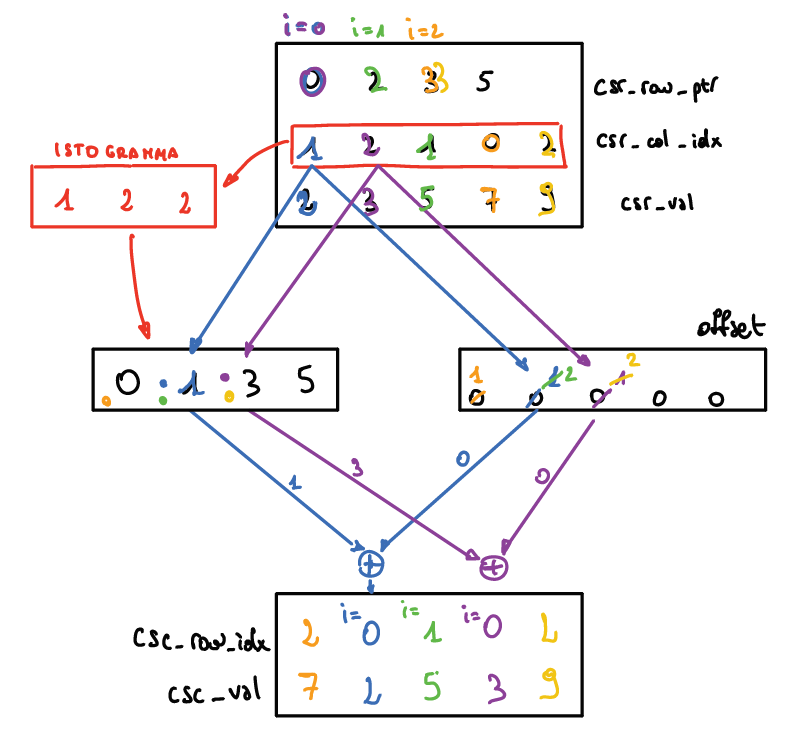
\includegraphics[scale=0.5]{transpose_algo_serial.PNG}
	\caption{Algoritmo seriale}
	\label{transpose_algo_serial}
\end{figure}

L'algoritmo si sviluppa nel seguente modo:
\begin{enumerate}
    \item si applica la funzione \emph{istogramma} \var{csr\_col\_idx} che calcola le occorrenze di ogni colonna, applicando \emph{scan} si ottiene il vettore \var{csc\_col\_ptr} (lunghezza $\mathrm{n}+1$) che conterrà i puntatori agli elementi di inizio riga trasposta;
    \item allochiamo il vettore \var{csc\_row\_idx} contente gli indici di riga (lunghezza $\mathrm{nnz}$);
    \item allochiamo il vettore \var{csc\_val} contente gli elementi non nulli (lunghezza $\mathrm{nnz}$);
    \item per ogni riga $i \in [0, m)$ processiamo gli elementi corrispondenti all'$i$-esima riga, legati alle posizioni $j \in [\var{csr\_row\_ptr}[i], \var{csr\_row\_ptr}[i+1])$
    \begin{itemize}
        \item la locazione $\mathrm{loc}$ del $j$-esimo elemento ordinata per righe è $\var{csr\_col\_ptr}[j] + \mathrm{offset}[j]$ dove $\mathrm{offset}[j]$ è un contatore incrementato ogni volta che aggiungiamo un elemento della colonna $\var{csr\_col\_ptr}[j]$;
        \item l'indice di riga dell'elemento $\mathrm{loc}$-esimo è $i$;
        \item il valore dell'elemento  $\mathrm{loc}$-esimo è $\var{csr\_val}[j]$.
    \end{itemize}
\end{enumerate}

L'esecuzione dell'algoritmo seriale è illustrato in Figura~\ref{transpose_algo_serial}.

\subsection{ScanTrans}

\begin{figure}[htbp]
    \centering
	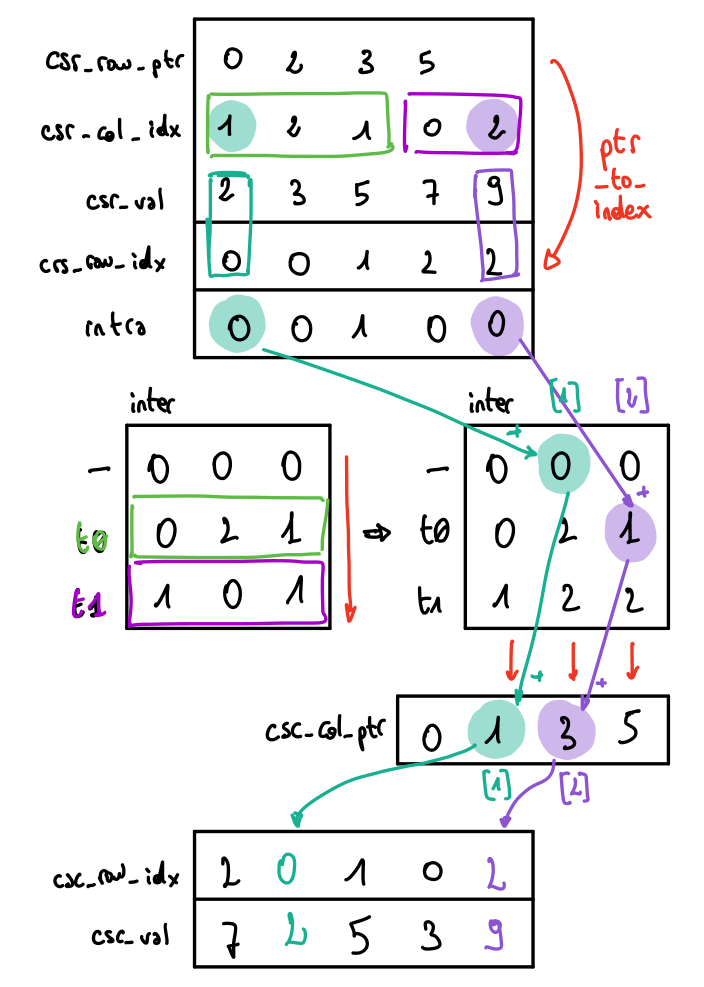
\includegraphics[scale=0.3]{transpose_scantrans.png}
	\caption{Algoritmo \ScanTrans}
	\label{transpose_algo_scantrans}
\end{figure}


L'algoritmo considerato prevede di effettuare la trasposta di matrici basandosi sul concetto di scan. Partendo sempre dal presupposto di avere in input una matrice in formato \textit{Csr}, vengono costruiti due array ausiliari:
\begin{itemize}
	\item inter: array bidimensionale di dimensione $ (nthreads+1) * n $,
	\item intra: array monodimensionale di dimensione massima $ nnz $.
\end{itemize}
Ogni riga in \textit{inter} contiene il numero di indici della colonna presi dalla thread i-esima. Mentre ogni elemento in \textit{intra} viene utilizzato per salvare l'offeset relativo alla colonna corrispondente all'elemento nnz preso dalla thread. Dopo aver ottenuto gli istogrammi, viene applicato un \textit{vertical scan} su inter, e una \textit{prefix sum} solamente sull'ultima riga di inter. Infine l'algoritmo calcola l'offset assoluto relativo ad ogni elemento nnz e ritorna il tutto in formato \textit{csc}.

Tutte le procedure utilizzate in \textit{Scan Trans} si trovano in sezione \ref{procedure}, e vengono eseguite nel seguente ordine:
\begin{enumerate}
	\item pointers to index: \ref{pnt-to-idx},
	\item index to pointers: \ref{idx-to-pnt},
	\item scan: \ref{scan},
	\item reorder elements.
\end{enumerate}

%\begin{figure}[H]
%	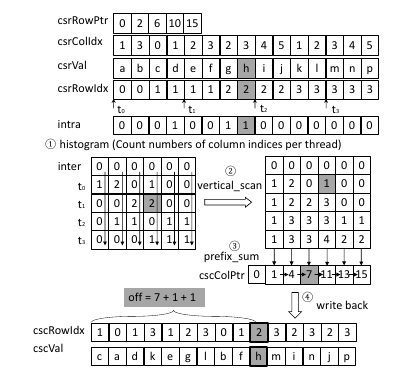
\includegraphics[scale=0.6]{scantrans.png}
%	\caption{Scan Trans, esempio utilizzato in \cite{parallelTrans}.}
%	\label{scantrans}
%\end{figure}

\subsection{MergeTrans}

\begin{figure}[htbp]
    \centering
	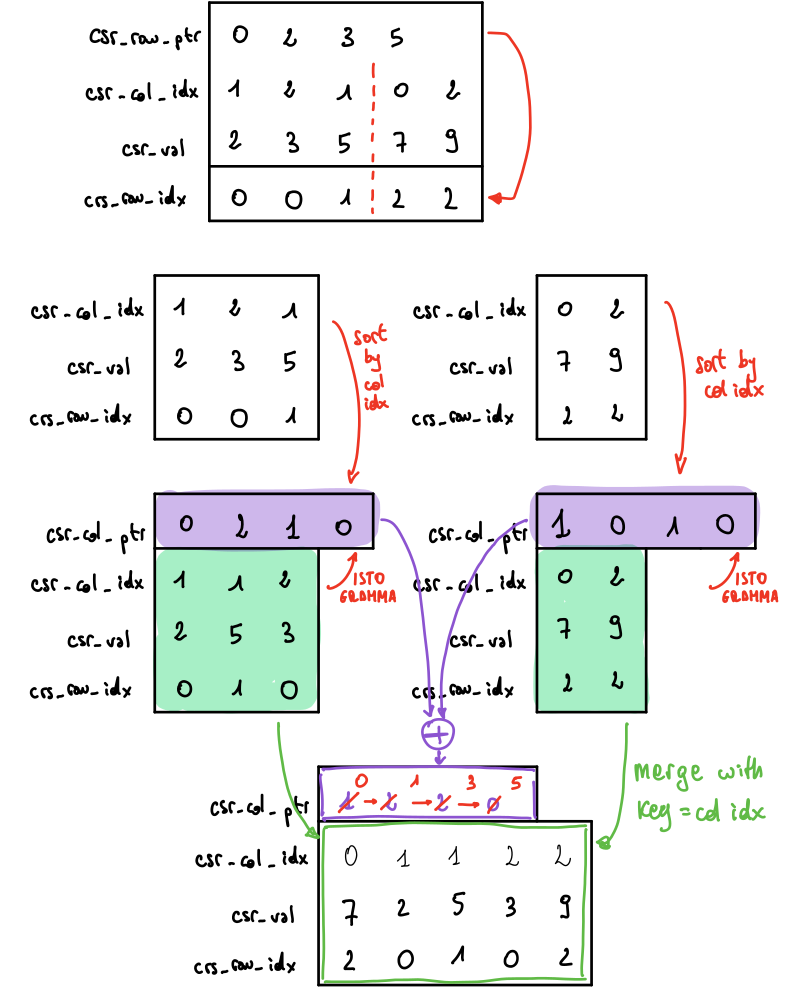
\includegraphics[scale=0.3]{transpose_mergetrans.png}
	\caption{Algoritmo \MergeTrans}
	\label{transpose_algo_scantrans}
\end{figure}
	
L'algoritmo considerato prevede due passi importanti: \textit{sort} e \textit{merge}.
Inizialmente sono stati creati gli indici di riga a partire dai puntatori delle colonne e su questi ultimi è stato fatto un sort su piccole porzioni di array, mantenendo quindi i vari blocchi disordinati tra di loro ma con gli elementi ordinati. Successivamente è stato utilizzato il merge ricorsivo partendo dai blocchi più piccoli e unendoli in blocchi sempre più grandi. Per funzionare questo processo necessita dell'utilizzo di due buffer di memoria che contengono gli elementi appena ordinati. Infine dai puntatori delle colonne vengono estraxtti gli indici e viene fatta la scan che ritorna il risultato in formato \textit{csc}. \newline
Anche in questo caso le procedure utilizzate si trovano in sezione \ref{procedure}, e sono ordinatamente eseguite come segue:
\begin{enumerate}
	\item pointers to index: \ref{pnt-to-idx},
	\item segmented sort: \ref{seg-sort},
	\item segmented merge: \ref{merge},
	\item index to pointers: \ref{idx-to-pnt},
	\item scan: \ref{scan}.
\end{enumerate}

%\begin{figure}[H]
%	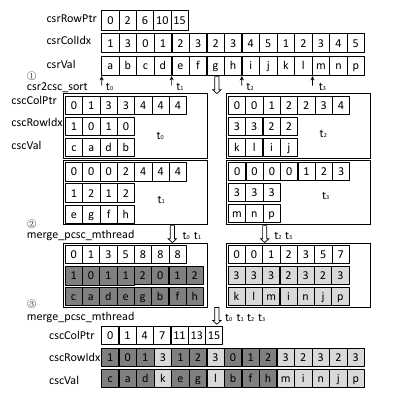
\includegraphics[scale=0.6]{mergetrans.png}
%	\caption{Merge Trans, esempio utilizzato in \cite{parallelTrans}.}
%	\label{mergetrans}
%\end{figure}


\subsection{Nvidia cuSPARSE}

Questo toolkit è implementato all'interno nelle librerie NVIDIA CUDA runtime. Le routine delle librerie vengono utilizzate per operazioni tra vettori e matrici che sono rappresentate tramite diversi formati. Inoltre mette a disposione operazioni che permettono la conversione attraverso diverse rappresentazioni di matrici. Supporta inoltre la compressione in formato \textit{csr} che è una delle più usate quando si vuole rappresentare matrici sparse in modo efficiente.

Il codice è stato sviluppato partendo dalla guida \cite{cusparse} ed è diviso in due versioni di cuSPARSE a causa delle Gpu utilizzate. In fase di compilazione viene quindi controllata la versione usata: $ 9 $ o $ 10 $.

Nel caso in cui la versione usata sia la $ 10 $ vengono svolti alcuni ulteriori passi, come l'allocazione dello spazio necessario per l'esecuzione di cuSparse oltre all'allocazione del buffer per il calcolo della trasposta. Per quanto riguarda la versione $ 9 $ invece questi passi non sono necessari.

Infine viene chiamata la procedura che effettua il calcolo della trasposta. Nel caso in cui la versione di cuSPARSE sia la $ 10 $ viene richiesto come ulteriore parametro l'algoritmo da utilizzare.\newline
Dopo essere state eseguite entrambe ritornano i valori ottenuti in formato \textit{csc}.
